\subsubsection{Vimdiff colors}

The default colors of \code{vimdiff} can be really bad because of the translation from 16-bit colors to 256-bit colors.

Code can be found here:

\url{https://github.com/robinhellmers/computer_setup/}

\begin{figure}[H]
    \centering
    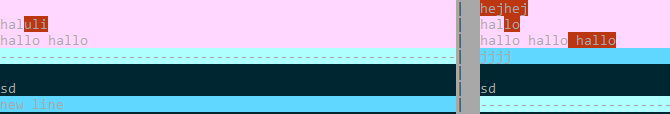
\includegraphics[width = \textwidth]{Figures/WSL/colors_vimdiff_defualt.PNG}
\end{figure}

This can be fixed to something like this instead:

\begin{figure}[H]
    \centering
    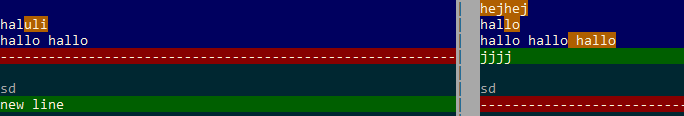
\includegraphics[width = \textwidth]{Figures/WSL/colors_vimdiff_customized.PNG}
\end{figure}

\begin{enumerate}
    \item Create the \code{~/.vim/colors/} directory. 
    \item Create a file \code{mycolorscheme.vim} in \code{~/.vim/color/}.
    \item Paste this into the file (see \href{https://github.com/robinhellmers/computer_setup/blob/master/mycolorscheme.vim}{Github}):
    
\begin{minted}[tabsize=3,obeytabs,linenos,bgcolor=codegray]{bash}
highlight DiffAdd    cterm=bold ctermfg=15 ctermbg=22 gui=none guifg=bg guibg=Red
highlight DiffDelete cterm=bold ctermfg=15 ctermbg=88 gui=none guifg=bg guibg=Red
highlight DiffChange cterm=bold ctermfg=15 ctermbg=17 gui=none guifg=bg guibg=Red
highlight DiffText   cterm=bold ctermfg=15 ctermbg=130 gui=none guifg=bg guibg=Red
\end{minted}

    \begin{itemize}
        \item \code{ctermfg} = foreground/text color
        \item \code{ctermbg} = background/highlight color
        \item Values given by xterm256 color table. This table might not correspond exactly to what you see on screen. Thereby it is better to print them out manually.
    \end{itemize}
    \begin{figure}[H]
        \centering
        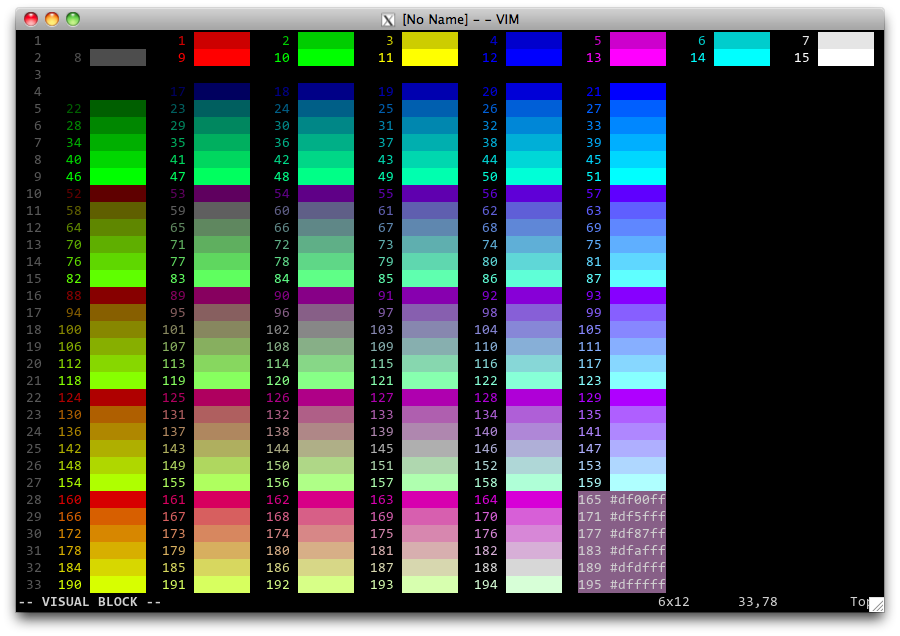
\includegraphics[width = \textwidth]{Figures/WSL/xterm256_color_table.png}
    \end{figure}
    \begin{enumerate}
        \item Create a file \code{color\_demo.vim} anywhere.
        \newpage
        \item Paste this into the file (see \href{https://github.com/robinhellmers/computer_setup/blob/master/color_demo.vim}{Github}):
        
\begin{minted}[tabsize=3,obeytabs,linenos,bgcolor=codegray]{vim}
let num = 255
while num >= 0
    exec 'hi col_'.num.' ctermbg='.num.' ctermfg=white'
    exec 'syn match col_'.num.' "ctermbg='.num.':...." containedIn=ALL'
    call append(0, 'ctermbg='.num.':....')
    let num = num - 1
endwhile
\end{minted}

    \item Open it up with \code{vim color\_demo.vim} and then use the command \code{:so color\_demo.vim}.
    \item This shows the background colors with corresponding values. Use \textbf{Page Up} and \textbf{Page down} to go through it.
        \begin{figure}[H]
            \centering
            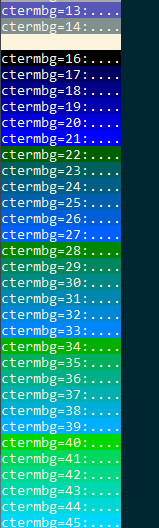
\includegraphics[width = 0.2\textwidth]{Figures/WSL/colors_demo.PNG}
        \end{figure}
    \end{enumerate}
    \item You can continuously edit \code{~/.vim/colors/mycolorscheme.vim} and see the updates of the colors while still in \code{vimdiff} by using the command \code{:colo mycolorscheme}.
    \item Now we are going to set this scheme permanently for \code{vimdiff}. Create a file in your home directory \code{~/.vimrc}.
    \newpage
    \item Paste this into the file (see \href{https://github.com/robinhellmers/computer_setup/blob/master/.vimrc}{Github}):
    
\begin{minted}[tabsize=3,obeytabs,linenos,bgcolor=codegray]{bash}
if &diff
    colorscheme mycolorscheme
endif
\end{minted}

\item Now the custom color scheme should be applied every time you open \code{vimdiff}.

\end{enumerate}